\documentclass[TA.tex]{subfiles}

\begin{document}


%\hyphenation{equi-va-len-cia}\hyphenation{pro-pie-dad}\hyphenation{res-pec-ti-va-men-te}\hyphenation{sub-es-pa-cio}

\chapter{Homología}

Para nociones de homología simplicial, consultar los apuntes de Homología Simplicial. Atención: en homología ordenada no existen los símplices en orden distinto al prefijado, no se toma cociente. 
\section{Homología singular}

Dado un espacio topológico $X$, definimos un $n$-\emph{símplice singular} como una aplicación continua $\sigma_n:\Delta^n\to X$, donde $\Delta^n$ es el $n$-símplice estándar. Denotamos $C_n(X)$ al grupo abeliano libre de todos los $n$-símplices singulares. A las combinaciones de la forma $\sum_{i=1}^n\lambda_i\sigma_n^i$ con $\lambda_i\in\Z$ se las llama $n$-\emph{cadenas} (estos son de hecho todos los elementos de $C_n(X)$. Tenemos definido también el operador borde $d_n:C_n(X)\to C_{n-1}(X)$, que es un homomorfismo de grupos abelianos definido como $d_n(\sigma_n)=\sum_{i=0}^n \sigma_n|_{[v_0,\dots, \hat{v_i},\dots, v_n]}$. Este operador verifica las mismas propiedades que el operador borde entre complejos simpliciales, con idéntica demostración. Así que hemos construido un complejo de cadenas singulares $\{C_n(X), d_n\}_{n\geq 1}=C_*(X)$. En caso de usar coeficientes en un grupo $G$ se indicará como $C_*(X,G)$. Análogamente a la homología simplicial, si $z\in C_n(X)$ y $d(z)=0$, decimos que $z$ es un $n$-ciclo. Si $z=d_{n+1}(z')$ para algún $z'\in C_{n+1}(X)$, decimos que $z$ es un $n$-borde. Como tenemos $B_n(X)=\Ima d_{n+1}\subseteq \ker d_n=Z_n(X)$, definimos el $n$-ésimo grupo de homología singular $H_n(X)=Z_n(X)/B_n(X)$. 


\begin{prop}
Si $X=\sqcup X_i$ (cantidad finita) es una descomposición de $X$ en sus componentes conexas por caminos, entonces $H_n(X)\cong \oplus_i H_n(X_i)$. 
\end{prop}
\begin{dem}
Como un símplice singular siempre tiene imagen conexa por caminos, $C_n(X)$ se escribe como suma directa de $C_n(X_i)$. Como $d_n$ respeta esta descomposición, $\ker d$ e $\Ima d$ se descomponen de la misma forma, por lo que $H_n(X)\cong \oplus_i H_n(X_i)$. \QED
\end{dem}

\begin{prop}\label{2.7}
Si $X\neq\emptyset$ es arco-conexo, entonces $H_0(X)\cong\Z$. 
\end{prop}
\begin{dem}
Por definición $H_0(X)=Z_0(X)/B_0(X)=C_0(X)/Ima d_1$. Definimos una aumentación $\varepsilon:C_0(X)\to\Z$ como $\varepsilon(\sigma_0)=1$ para todo 0-símplice singular. Como $X\neq\emptyset$, $\varepsilon$ es sobreyectivo, porque podemos un el 0-símplice. Vamos a probar que $\ker\varepsilon=\Ima d_1$, con lo que usando el primer teorema de isomorfía tendremos que $H_0(X)\cong \Ima\varepsilon=\Z$. 

Veamos primero $\Ima d_1\subseteq\ker\varepsilon$. Sea $\sigma_1:\Delta^1\to X$, entonces $\varepsilon(d_1(\sigma_1))=\varepsilon(\sigma_1|_{v_1})-\varepsilon(\sigma_1|_{v_0})=0$.

Ahora la inclusión contraria, $\ker\varepsilon\subseteq\Ima d_1$. Sea $z\in C_0(X)$ tl que $\varepsilon(z)=0$. Por definición $z=\sum_{i=1}^k \lambda_i\sigma^i$, donde $\sigma_i$ son aplicaciones constantes $x_i$. Entonces $\varepsilon(z)=\sum_{i=1}^k\lambda_i$. Consideramos los 1-símplices singulares $\tau_i$ que son un camino entre $x_0$ y $x_i$ y definimos $\tau=\sum_{i=1}^k\lambda_i\tau_i\in C_1(X)$. Entonces
\[
d_1(\tau)=\sum_{i=1}^k \lambda_id(\tau_i)=\sum_{i=1}^k \lambda_i(x_i-x_0)=\sum_{i=1}^k\lambda_i\sigma_i-(\sum_{i=1}^k\lambda_i)x_0
\]
Como $\sum_{i=1}^k\lambda_i=0$ por ser $\varepsilon(z)=0$,  $d_1(\tau)=z$. \QED
\end{dem}

\begin{prop}
Si $X$ es un punto, entonces $H_n(X)=0$ para $n>0$ y $H_0(X)=\Z$.
\end{prop}

\begin{dem}
$H_0(X)=\Z$ se tiene por ser $X$ arco-conexo. Para el resto de caso miramos directamente el complejo de cadenas. $C_n(X,\Z)$ tiene solamente un $n$-símplice singular $\sigma_n$, y el operador borde $d(\sigma_n)=\sum_i (-1)^i\sigma_{n-1}$, que es 0 para $n$ impar y $\sigma_{n-1}$ para $n$ par. Entonces tenemos el complejo de cadenas
\[
\cdots\Z\xrightarrow{\cong}\Z\xrightarrow{0}\Z\xrightarrow{\cong}\Z\xrightarrow{0}\Z\to 0
\]
cuya homología es trvial para $n>0$. 
\QED
\end{dem}

Una variación del complejo de cadenas singulares es el complejo de cadenas singulares aumentado, definiendo $\varepsilon:C_0(X)\to \Z$ como $\varepsilon(\sigma_0)=1$ para todo 0-símplice singular. Denotamos como $\widetilde{C}_n$ a los grupos de este complejo, que en realidad coinciden en todos los niveles salvo en -1, que es $\Z$. Hemos visto en la demostración de la proposición \ref{2.7} que $\varepsilon d_1=0$, así que podemos definir la homología reducida con valor
\[
\widetilde{H}_n(X)=\begin{cases}
H_n(X) & n>0\\
H_0(X)/\Z & n=0
\end{cases}
\]
El primer caso es trivial, vamos a probar el segundo, aunque usaremos algunas nociones de álgebra que veremos más adelante.  Tenemos el diagrama conmutativo
\[
\begin{tikzcd}
\ker\varepsilon\arrow[rd,twoheadrightarrow]\arrow[r,twoheadrightarrow] & \ker\overline{\varepsilon}\arrow[r, rightarrowtail]& H_0(X)\arrow[d, twoheadrightarrow, "\overline{\varepsilon}"]\\
C_1(X)\arrow[r, "d_1"]\arrow[d, twoheadrightarrow] & C_0(X)\arrow[r, twoheadrightarrow, "\varepsilon"]\arrow[ur,twoheadrightarrow]  & \Z\\
\Ima{d_1}\arrow[ur, rightarrowtail]
\end{tikzcd}
\]
donde $\overline{\varepsilon}$ es la aplicación inducida en $H_0(X)$ por $\varepsilon$ (es fácil comprobar que está bien definida). El hecho de que $\varepsilon\circ d_1=0$ nos proporciona además $\Ima d_1 \rightarrowtail\ker\varepsilon$. Esto nos da la sucesión exacta corta
\[
\Ima d_1 \rightarrowtail\ker\varepsilon\twoheadrightarrow\ker\overline{\varepsilon}
\]
El primer teorema de isomorfía nos da además $\ker\overline{\varepsilon}\cong \ker\varepsilon/\Ima d_1=\widetilde{H}_0(X)$. Así sustituyendo en el diagrama anterior obtenemos la sucesión exacta corta
\[
\widetilde{H}_0(X)\rightarrowtail H_0(X)\overset{\overline{\varepsilon}}{\twoheadrightarrow}\Z
\]
Como el grupo de la derecha es abeliano libre, la sucesión escinde, con lo que $H_0(X)=\Z\oplus \widetilde{H}_0(X)$.

%$\twoheadleftarrow \twoheadrightarrow \rightarrowtail \leftarrowtail$

\subsection{Invariancia homotópica}

%f_\sharp

Si tenemos una aplicación continua $X\to Y$, se induce una aplicación $f_*: C_n(X)\to C_n(Y)$ definido como $\sigma\mapsto f\circ\sigma$, que conmuta con el operador borde (es un morfismo de complejos de cadenas), como vamos a comprobar.  Si $\sigma\in C_n(X)$, 
\[
f_*(d_n(\sigma))=\sum_{i=0}^n (-1)^i (f\circ\sigma)|_{[v_0,\dots, \hat{v_i}, \dots, v_n]}=d_n(f\circ\sigma)
\]

Esto implica que si $z\in C_n(X)$ con $d(z)=0$, entonces $d_n(f_*(z))=f_*(d_n(z))=0$, por lo que $f_*$ envía ciclos en ciclos. De igual manera, envía bordes en bordes. De este modo, se induce un homomorfismo dentado igual, $f_*:H_n(X)\to H_n(Y)$. 

Además $(g\circ f)_*=g_*\circ f_*$ y $(Id_X)_*=Id_*$ tanto en complejos de cadenas como en homología.


\begin{teorema}
Si $f,g:X\to Y$ son continuas con $f\simeq g$, entonces $f_*=g_*:H_n(X)\to H_n(Y)$ para todo $n\geq 0$. 
\end{teorema}\
 \opencutright
\begin{dem}
%This is where the table goes with text wrapping around it. You may 
%embed tabular environment inside wraptable environment and customize as you like.

%------------------------------------------
%\begin{wrapfigure}{r}{4cm}
%\caption{A wrapped figure going nicely inside the text.}\label{wrap-fig:1}
%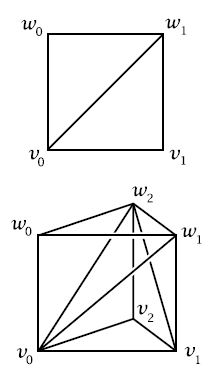
\includegraphics[width=4cm]{cilindrosimplice}
%\end{wrapfigure} 
%------------------------------------------
\def\windowpagestuff{\flushright 
   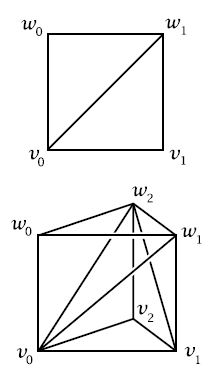
\includegraphics[width=2.8cm,height=4.5cm]{cilindrosimplice}}
   
  
   \begin{cutout}{1}{0.75\textwidth}{0pt}{6}
     \noindent
El primer paso será subdividir $\Delta^n\times I$ en simplices. Sea $\Delta^n\times\{0\}=[v_0,\dots, v_n]$ y $\Delta^n\times\{1\}=[w_0,\dots, w_n]$, donde $v_i$ tiene la misma imagen que $w_i$ mediante la proyección $\Delta^n\times I\to \Delta$. Para cada $0\leq i\leq n$ consideramos el $(n-1)$-símplice $[v_0,\dots, v_i, w_i,\dots, w_n]$. Este símplice se ha conseguido simplemente recorriendo $\Delta^n\times\{0\}$ hasta el vértice $v_i$ y después saltando a $w_i$ para recorrer el resto de $\Delta^n\times\{1\}$, para luego volver a $v_0$. La figura muestra los casos $n=1,2$.
\end{cutout}\
%INTENTAR CON CUTWIN \url{https://tex.stackexchange.com/questions/40806/how-to-wrap-text-around-a-figure-revised}
%\begin{figure}[h!]
%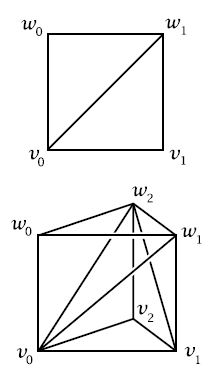
\includegraphics[scale=0.7]{cilindrosimplice}
%\end{figure}

Dada una homotopía $F:X\times I\to Y$ y un símplice singular $\sigma:\Delta^n\to X$, podemos formar la composición $F\circ(\sigma\times Id):\Delta^n\times I\to X\times I\to Y$. Usando esto podemos definir el \emph{operador prisa} $P:C_n(X)\to C_{n+1}(Y)$ como sigue
\[
P(\sigma)=\sum_i(-1)^iF\circ(\sigma\times I)|_{[v_0,\dots, v_i, w_i,\dots, w_n]}
\]
Vamos a demostrar que el operador prisma satisface la relación
\[
dP=g_*-f_*-Pd
\]
Para probarlo calculamos
\[
dP(\sigma)=\sum_{j≤i}
(−1)^i(−1)^jF\circ(σ \times Id)|_{ 
[v_0, \dots, \hat{v}_j , \dots ,v_i,w_i, \dots ,w_n]}
+\sum_{j≥i}
(−1)^i(−1)^{j+1}F\circ(σ\times Id)|_{
[v_0, \dots ,v_i,w_i, \dots ,\hat{w}_j , \dots ,w_n]}
\]
Los términos para $i=j$ se cancelan excepto para $F\circ(σ \times Id)|_{ 
[\hat{v}_0,w_0,\dots ,w_n]}$, que es $g\circ\sigma=g_*(\sigma)$; y $-F\circ(σ \times Id)|_{ 
[v_0,,\dots ,v_n,\hat{w}_n]}$, que es $-f\circ \sigma=-f_*(\sigma)$. Los términos para $i\neq j$ son exactamente $-Pd(\sigma)$. 

Así, si $\alpha\in Z_n(X)$, entonces $g_*(\alpha)-f_*(\alpha)=Pd(\alpha)+dP(\alpha)=dP(\alpha)$ por ser $d\alpha=0$. Entonces $g_*(\alpha)$ y $f_*(\alpha)$ determinan la misma clase de homología al ser su diferencia un borde. 
%Para el caso aumentado creo que P=0 (comprobar).
\end{dem}

En la prueba hemos usado la relación $dP-Pd=f_*-g_*$, que es la que define una \emph{homotopía de complejos de cadenas} entre $f_*$ y $g_*$ (se denota en ese caso $f_*\simeq g_*$). Una \emph{equivalencia de homotopía} enre complejos de cadenas $f:C_*\to D_*$ es un morfismo de complejos de cadenas tal que existe $g:D_*\to C_*$ de modo que $g\circ f\simeq Id_{C_*}$ y $f\circ g\simeq Id_{D_*}$.  Hemos probado además que una equivalencia de homotopía de complejos de cadenas induce isomorfismo en la homología. Para el caso de homología reducida también es válido este resultado definiendo $f_*:\Z\to\Z$ como 0 y $P:\Z\to C_0(Y)$ como la aplicación nula.

\begin{coro}
Si $f:X\to Y$ es equivalencia homotópica, entonces $f_*$ es isomorfismo.
\end{coro}

\section{Álgebra Homológica}

Asumimos conocidas las definiciones y propiedades básicas de las sucesiones exactas. 

\begin{lemma}[Splitting lemma]
Dada una sucesión exacta de módulos $0\to A\xrightarrow{f}B\xrightarrow{g}C\to 0$ son equivalentes:
\begin{enumerate}[a)]
\item Hay un morfismo $p:B\to A$ tal que $pf=Id:A\to A$.
\item Hay un morfismo $s:C\to B$ tal que $gs=Id:C\to C$. 
\item Existe un isomorfismo $B\cong A\oplus C$ compatible con la sucesión exacta corta, es decir, que hace conmutar el siguiente diagrama
\[
\begin{tikzcd}
A\arrow[r, rightarrowtail, "f"]\arrow[d, equals] & B\arrow[r, twoheadrightarrow, "g"]\arrow[d, "u"] & C\arrow[d, equals] \\
A\arrow[r, "i"] & A\oplus C\arrow[r, "\pi"]& C
\end{tikzcd}
\]
\end{enumerate}
\end{lemma}
\begin{proof}
Que c) implica a) y b) es trivial.

Para ver que a) implica c), sea $p:B\to A$ un homomorfismo que verifique $pf=Id$. En este caso, afirmamos que $B=f(A)\oplus\ker p$. Si $b\in B$, entonces $b=fp(b)+(m-fp(b))$. Es claro que $fp(b)\in f(A)$ y además $p(b-fp(b)=p(b)-pfp(b)=p(b)-p(b)=0$, luego $b-fp(b)\in\ker p$. Se tiene también que si $b\in f(A)\cap\ker p$, entonces $b=f(a)$ y $0=p(b)=pf(a)=a$, por lo que $b=0$, con lo que la afirmación es cierta. Una vez que tenemos $b=f(a)+b'$, definimos el homomorfismo $u(b)=a+g(b')$. Se tiene de hecho que $u(b)=a+g(b)$, pues si $b-b'=f(a)$ y por exactitud $g(b-b')=0$. Esta definición no es ambigua por ser $f$ inyectiva. Por la definición que se ha hecho, el diagrama es conmutativo y el lema de los 5 implica que $u$ es isomorfismo.

Por último veamos que b) implica c). Sea $s:C\to B$ tal que $gs=Id$. Afirmamos que $B=\ker g\oplus s(C)$. Sea $b\in B$, lo escribimos como $b=(b-sg(b))+sg(b)$. Es claro que $sg(b)\in s(C)$ y además $g(b-sg(b))=g(b)-gsg(b)=g(b)-g(b)=0$, por lo que $b-sg(b)\in\ker g$. Si $b\in\ker g\cap s(C)$, entonces $b=s(c)$ y $0=g(b)=gs(c)=c$, por lo que $b=0$, lo que prueba la afirmación. Ahora, como $\ker g=\Ima f$, podemos expresar $b=f(a)+s(c)$. Definimos entonces $u(b)=a+c$, lo cual tiene sentido porque tanto $f$ como $s$ son inyectivas y además $\Ima s\cap\Ima f=\Ima s\cap\ker g=0$. La definición que hemos hecho hace conmutar el diagrama y esto hace que $u$ sea isomorfismo por el lema de los cinco. 
\end{proof}

Cuando $C$ es un objeto proyectivo se verifica la escisión. En particular, cuando sea un objeto libre. Se recuerda que una sucesión de complejos  de cadenas $0\to A^*\to B^*\to C^*\to 0$ se dice exacta si lo es en cada nivel. Se advierte que el hecho de que se tenga escisión en cada nivel no implica que $B^*\cong A^*\oplus C^*$ pues los isomorfismos de cada nivel no tienen por qué ser compatibles con el operador borde. 

\begin{teorema}
Toda sucesión exacta corta de complejos de cadenas $0\to A\xrightarrow{f} B\xrightarrow{g} C\to 0$ induce una sucesión exacta larga
\[
\cdots \to H_n(A)\xrightarrow{f_*}H_n(B)\xrightarrow{g_*}H_n(C)\xrightarrow{\partial}H_{n-1}(A)\to\cdots
\] 
%\xrightarrow[g] pone la g debajo
\end{teorema}
La prueba sigue la clásica estrategia de \emph{diagram chasing} y se puede encontrar a partir de la página 116 de \emph{Algebraic Topology} de Allen Hatcher. 
\section{Homología relativa}

Dado un subespacio $A\subseteq X$, vamos a construir el complejo de cadenas relativo $C_*(X,A)$ asociado al par $(X,A)$, lo que nos dará la homología relativa $H_*(X,A)$. Esto se consigue definiendo $C_n(X,A)=C_n(X)/C_n(A)$. Este cociente tiene sentido porque $A\subseteq X$ y entonces el complejo está contenido mediante la aplicación inducido por la inclusión. Como $d$ lleva $C_n(A)$ en $C_{n-1}(A)$, podemos definir $d:C_n(X,A)\to C_{n-1}(X,A)$ como $d([x])=[d(x)]$. Así, la homología relativa es la homología del complejo de cadenas $H_n(X,A)=H_n(C_*(X,A))$. 

A partir de las sucesión exacta corta evidente $0\to C_*(A)\to C_*(X)\to C_*(X,A)\to 0$ surge la sucesión exacta larga de homología relativa
\[
\cdots \to H_n(A)\xrightarrow{f_*}H_n(X)\xrightarrow{g_*}H_n(X,A)\xrightarrow{\partial}H_{n-1}(A)\to\cdots
\]

También existe el análogo reducido de esta sucesión exacta larga para un par $(X,A)$ donde $A\neq\emptyset$, obtenida a partir de las sucesiones exactas cortas $0\to C_n(A)\to C_n(X)\to C_n(X,A)\to 0$ aumentadas en dimensión $-1$ por $0\to\Z\xrightarrow{Id}\Z\to 0\to 0$. En particular, esto significa que $\widetilde{H}_n(X,A)=H_n(X,A)$ para todo $n$ si $A\neq\emptyset$.

\begin{defi}
Una aplicación de pares $f:(X,A)\to (Y,B)$ es una aplicación $f:X\to Y$ tal que $f(A)\subseteq B$. 
\end{defi}

Una aplicación de pares induce una aplicación $f|_A:A\to B$, así que se puede definir un morfismo de complejos de cadenas inducido por $f$, $f_*:C_*(X,A)\to C_*(Y,B)$ como $[c]\mapsto [f_*(c)]$ que cumple las propiedades de funtorialiad. Por tanto da lugar también a un homomorfismo en homología $f_*:H_*(X,A)\to H_*(Y,B)$, que es natural con respecto a la sucesión exacta larga de homología relativa, es decir, conmuta el diagrama 
\[
\begin{tikzcd}
\cdots \to H_n(A)\arrow[r]\arrow[d, "f|_{A*}"] & H_n(X)\arrow[r]\arrow[d, "f_*"] & H_n(X,A)\arrow[d, "f_*"]\arrow[r] &H_{n-1}(A)\arrow[d]\to\cdots\\
\cdots \to H_n(B)\arrow[r] & H_n(Y)\arrow[r] & H_n(X,B)\arrow[r]& H_{n-1}(B)\to\cdots
\end{tikzcd}
\]

ya que la conmutatividad se tiene ya a nivel de complejos de cadenas, y la conmutatividad con $\partial$ se puede probar. 
 

\begin{teorema}[de excisión]\label{excision}
Sean subespacios $Z\subseteq A\subseteq X$ tal que la clausura de $Z$ está en el interior de $A$. Entonces la inclusión $i:(X-Z,A-Z)\hookrightarrow (X,A)$ induce isomorfismos $i_*:H_n(X-Z,A-Z)\to H_n(X,A)$ para todo $n$. Equivalentemente, para subespacios $A,B\subseteq X$ cuyos interiores cubren $X$, la inclusión $(B,A\cap B)\hookrightarrow (X,B)$ induce isomorfismos $H_n(B,A\cap B)\to H_n(X,B)$ para todo $n$. 
\end{teorema}

Para un espacio $X$, consideremos una familia de subconjuntos $\mathcal{U}=\{U_i\}_{i\in I}$ tales que $X=\cup_i int(U_i)$. Decimos que un símplice singular en $X$, $\sigma:\Delta^n\to X$ está \emph{subordinado} a $\mathcal{U}$ si existe $I\in I$ con $\delta(\Delta^n)\subseteq U_i$. Denotamos $C^{\mathcal{U}}_*$ al complejo de cadenas de símplices de $X$ subordinados a $\mathcal{U}$, que está contenido en $C_*(X)$.  El operador borde está bien definido, puesto que si $\sigma:\Delta^n\to X$ es tal que $\sigma(\Delta^n)\subseteq U_i$ y si $\Delta^n_i$ es la $i$-ésima cara de $\Delta^n$, entonces $d(\sigma)=\sum_{i=0}^n(-1)^i\sigma|_{\Delta^n_i}$. Como $\sigma(\Delta^n)\subseteq U_i$, también lo está la restricción a cada una de las caras.

\begin{teorema}[de las cadenas pequeñas]\label{peque}
La inclusión $C^{\UU}_*(X)\hookrightarrow C_*(X)$ es una equivalencia homotópica de complejos de cadenas. 
\end{teorema}

\begin{defi}
El \emph{baricentro} de un símplice $\sigma=[v_0,\dots, v_n]$ es $b(\sigma)=\sum_{i=0}^n\frac{1}{n+1}v_i\in \sigma$. La \emph{subdivisión baricéntrica} es el complejo simplicial formado por los baricentros de las caras de $\sigma$. La $k$-ésima subdivisión baricéntrica es la división baricéntrica de la $k-1$-ésima subvidisión baricéntrica.
\end{defi}

En general, si $\sigma$ es un símplice y dados $\sigma_0\leq\cdots\sigma_t\leq\sigma$, se tiene que $[b(\sigma_0),\dots, b(\sigma_t)]$ forma un símplice contenido en $\sigma$. 

Se define el \emph{diámetro} de $\sigma\subseteq \R^N$ como $dia(\sigma)=\max_{x,y\in\sigma} d(x,y)$. Denotamos $d(x,y)$ como $|x-y|$. Dados $x,y\in\sigma$, con $y=\sum_{i=0}^n t_iv_i$ y $\sum_{i=0}^nt_i=1$, 
\[
|x-y|=\left|\sum_{i=0}^nt_ix-\sum_{i=0}^nt_iv_i\right|=\left|\sum_{i=0}^nt_i(x-v_i)\right|\leq \sum_{i=0}^n t_i|x-v_i|\leq \sum_{i=0}^nt_i\max_{j=0,\dots, n}|x-v_j|=\max|x-v_j|\leq \max|v_k-v_j|
\]

\begin{lemma}
 Si $\tau$ es un símplice de la subdivisión baricéntrica de $\sigma$, $\dim(\sigma)=n$, 
\[
dia(\tau)\leq\frac{n}{n+1}dia(\sigma)
\]
\end{lemma}

La demostración se puede encontrar en los apuntes de Homología Simplicial o alternativamente en Hatcher página 120. 

\begin{coro}
Si $\tau$ es un símplice de la $k$-ésima subdivisión baricéntrica de $\sigma$, $\dim(\sigma)=n$, 
\[
dia(\tau)\leq \left(\frac{n}{n+1}\right)^k dia(\sigma)
\]
\end{coro}

\begin{coro}\label{r}
Sea $\sigma$ un $q$-símplice sobre $X$ y $\mathcal{P}$ un recubrimiento por abiertos de $X$. Entonces $\exists r>0$ tal que $S^r(\sigma)$ es combinación lineal de símplices subordinados a $\mathcal{P}$, esto es, si $\mathbb{P}=\{V_i\}_{i\in I}$, existe $i\in I$ con $\Ima\sigma\in V_i$. 
\end{coro}
\begin{dem}
$\sigma$ es una aplicación continua que parte de un espacio métrico compacto, luego $\{\sigma^{-1}(V_i)\}$ es recubrimiento de $\Delta^q$. Tomamos $\varepsilon>0$ el número de Lebesgue de $\Delta_q$ respecto de $\sigma^{-1}(\mathcal{P})$. Entones existe $r>0$ tal que el diámetro de $S^r(\Delta_q))$ es menor que $\varepsilon$, por lo que $S^r(\sigma)$ está subordinado a $\mathcal{P}$. 
\end{dem}

\begin{dem}[del teorema de Excisión]
No usamos la estrategia de Hatcher sino de Greenberg, usando que $C_*^{\UU}(X,A)\to C_*(X,A)$ induce isomorfismo en homología. Definimos un morfismo de complejos de cadenas $S:C_q(X)\to C_q(X)$ llamado \emph{subdivisión} y una homotopía de complejos de cadenas $T:C_*(X)\to C_{*+1}(X)$ entre la identidad y $S$, es decir $dT+Td=Id-S$, que funcionarán de forma natural (como functores). En particular, si $\sigma:\Delta^q\to X$, tenemos el diagrama conmutativo
\[
\begin{tikzcd}
C_q(\Delta^q)\arrow[r, "S_q"]\arrow[d, "\sigma_*"] & C_q(\Delta^q)\arrow[d, "\sigma_*"]\\
C_q(X)\arrow[r, "S_q"] & C_q(X)
\end{tikzcd}
\] 
Si consideramos la identidad $\delta:\Delta^q\to\Delta^q\in C_q(\Delta^q)$, $\sigma=\sigma_*(\delta)\in C_q(X)$, entonces $S_q(\sigma)=\sigma_*(S_q(\delta))$. 

Tendremos luego un cubo como el siguiente 
\[
\begin{tikzcd}
&
C_q(\Delta^q)
\ar{dl}[swap, sloped, near start]{\sigma_*}
\ar{rr}{S_q}
\ar[]{dd}[near start]{d}
& & C_q(\Delta^q)
\ar{dd}{d}
\ar{dl}[swap, sloped, near start]{\sigma_*}
\\
C_q(X)
\ar[crossing over]{rr}[near end]{S_q}
\ar{dd}[swap]{d}
& & C_{q}(X)
\ar[crossing over]{dd}[]{d}
\\
&
C_{q-1}(\Delta^q)
\ar[near start]{rr}{S_{q-1}}
\ar[sloped, swap]{dl}{\sigma_*}
& & C_{q-1}(\Delta^q)
\ar[sloped, swap]{dl}{\sigma_*}
\ar{dl}
\\
C_{q-1}(X)
\ar{rr}{S_{q-1}}
& & C_{q-1}(X)
\ar[crossing over, leftarrow, near start]{uu}{}
\end{tikzcd}
\]
en el que todas las caras salvo la frontal habrán sido probadas conmutativas, pero la conmutatividad de esta cara se deduce de la del resto.

Vamos a definir entonces $S$ y $T$ inductivamente. $S(\delta_0)=\delta_0=T(\delta_0)$. $S_q(\delta_q)=B_q(S_{q-1}d\delta_q)$, donde $B_q$ es el cono sobre la subdivisión baricéntrica de $d(\delta_q)$ (recordemos que $\Delta_q$ es el cono de $\Delta_{q-1}$, que podemos tomar con vértice extra un punto que tiene como proyección el baricentro de $\Delta_{q-1}$, y sobre una cadena no es más que una cadena de conos). Aunque no se vea muy intuitivo, a cada símplice le asocia la suma de los símplices de su subdivisión baricéntrica. $T_q(\delta_q)=B_q(\delta_q-S\delta_q-T_{q-1}(d\delta_q))$.

Veamos que $dS=Sd$. Si $q=0$, $dS=Sd=0$. Para $q>0$, 
\[
dS(\delta_q)=dS(\delta_q)=d(B_q(S_{q-1} d\delta_q))
\]
Ahora, $d(B\sigma)=\sigma-Bd\sigma$, pues $d([B,v_0,\dots, v_q])=[v_0,\dots, v_q]-Bd[v_0,\dots, v_q]$. Luego, aplicando hipótesis de inducción
\[
d(B_q(S_{q-1} d\delta_q))=S_{q-1}dS_q-B_q(dS_{q-1}d\delta_q)=S_{q-1}d\delta_q-B_qS_{q-1}ddS_q=S_{q-1}D(\delta_q)
\]

Ahora vemos que $dT+Td=Id-S$. 
\[
dT\delta_q=d(B_q(\delta_q-S\delta_q-TdS_q)=(\delta_q-S\delta_q+TdS_q)-B_q(d\delta_q-dS\delta_q-dTd\delta_q)=
\]
\[
(\delta_q-S\delta_q-Td\delta_q)-B_q(d\delta_q-Sd\delta_q-(d\delta_q-Sd\delta_q-Td(d\delta_q)))=
\]
\[
\delta_q-S\delta_q+Td\delta_q
\]

Tenemos ya entonces que $S_*=Id_*:H_q(X)\to H_q(X)$. Probamos ahora el siguiente resultado
\begin{lemma}
Sea $X$ un espacio topológico y $\mathcal{P}$ un recubrimiento por abiertos de $X$. Entonces, todo ciclo de $H_q(X,A)$ puede ser representado por un ciclo subordinado a $\mathcal{P}$.
\end{lemma}
\begin{proof}
Dado $[z]\in H_q(X,A)$, $z$ es un ciclo relativo, luego $d(z)$ es un borde relativo, así que es una cadena en $A$. Además $z-S(z)=dT(z)+Td(z)$. Se tiene que $Td(z)$ tiene imagen en $A$, luego $z\equiv S(z)+dT(z)\mod A$. Así que $[z]=[S(z)]\in H_q(X,A)$. Inductivamente obtenemos $[z]=S^r(z)]\in H_q(X,A)$, luego basta tomar $r>0$ como en el corolario \ref{r}. 
\end{proof}

Finalmente podemos probar que $i_*:H_q(X-Z,A-Z)\to H_q(X,A)$ es isomorfismo. Primero vemos que es sobreyectiva. Sea $[z]\in H_q(X,A)$, $z=\sum\lambda_i\sigma_i$ subordinado a $\{int A, X-\overline{Z}\}$, esto es, cualquier $\sigma_i$ cuya imagen no caiga en $X-Z\supseteq X-\overline{Z}$, verifica que su imagen cae en $int(A)\subseteq A$, luego los podemos eliminar. Podemos suponer entonces que $X$ cae $X-Z$, luego $[z]$ define una clase  en $H_q(X-Z,A-Z)$. 

Ahora probamos que $i_*$ es inyectiva. Si $[z]\in H_q(X-Z,A-Z)$ es tal que $i_*[z]=0\in H_q(X,A)$, esto quiere decir que $z=z'+dw$ para $w\in C_{q-1}(X,A)$ y $z'\in C_q(A)$. Elegimos $r>0$ de modo que $S^r(z)$ esté subordinado a $\{intA, X-\overline{Z}\}$. Así $S^r(z)=S^r(z')+d(S^r(w))$. Por un lado, $S^r(w)=w_q+w_2$, donde $w_1$ tiene símplices singulares en $X-\overline{Z}$ y $w_2$ en $int(A)$. De modo que $S^r(z)-dw_1=S^r(z')+dw_2$, donde el término de la izquierda está en $X-Z$ y el de la derecha en $A$, luego tienen que caer en $A-Z$. Así que $S^r(z)\simeq 0$ en $X-Z\mod A-Z$, es decir $[z]=[S^r(z)]=0\in H_q(X-Z,A-Z)$.  
\end{dem}


\begin{prop}
Si $f:(X,A)\to (Y,B)$ es una aplicación de pares tal que tanto $f:X\to Y$ como $f|_A:A\to B$ son equivalencias de homotopía, entonces $f$ como aplicación depares induce isomorfismos en homología relativa $f_*:H_n(X,A)\to H_n(Y,B)$ para todo $n\in\Z$.
\end{prop}
\begin{dem}
Es trivial a partir de las sucesiones largas de homología relativa respectiva, que equivalencias de homotopía inducen isomorfismos y el lema de los cinco.
\end{dem}

\begin{defi}
Un \emph{buen par} $(X,A)$ es un par tal que $A\subseteq X$ es cerrado y existe un abierto $U$ con $A\subseteq U\subseteq X$ tal que $A$ es retracto de deformación fuerte de $U$.
\end{defi}


\begin{prop}
Sea $X$ un espacio y $x_0\in X$. Entonces $\widetilde{H}_n(X)\cong\widetilde{H}_n(X,x_0)=H_n(X,x_0)$.
\end{prop}
\begin{dem}
Como $\widetilde{H}_*(x_0)=0$, al sustituir en la sucesión exacta larga de homología relativa tenemos los isomorfismos buscados.
\end{dem}

\begin{prop}\label{2.22}
Si $(X,A)$ es un buen par, entonces $(X,A)\to (X/A,A/A)$ induce isomorfismos $H_n(X,A)\cong H_n(X/A,A/A)\cong\widetilde{H}_n(X/A)$ para todo $n\in\Z$. 
\end{prop}
\begin{dem}
Consideremos el diagrama conmutativo siguiente.
\[
\begin{tikzcd}
H_n(X,A)\arrow[d,"p_*"]\arrow[r,"i_*"] & H_n(X,U)\arrow[d]&H_n(X-A,U-A)\arrow[l]\arrow[d]\\
H_n(X/A,A/A)\arrow[r, "i_*"]& H_n(X/A, U/A) &\arrow[l]H_n((X/A)-[A], (U/A)-[A])
\end{tikzcd}
\]
Se tiene que $i_*:H_n(X,A)\to H_n(X,U) $ es isomorfismo porque está inducido por la inclusión y $A$ es retracto de deformación fuerte de $U$. Esta retracción pasa al cociente y $[A]$ es retracto fuerte de $U/A$. Las flechas horizontales de la derecha son isomorfismos por excisión. Como la aplicación cociente es homeomorfismo fuera de $A$, la flecha vertical de la derecha es isomorfismo, al estar inducida por un homeomorfismo de pares. Por conmutatividad también es isomorfismo la flecha central. De nuevo por conmutatividad es isomorfismo $p_*$, que era lo que queríamos probar. 
\end{dem}

\begin{teorema}
Si $(X,A)$ es un buen par, entonces tenemos una sucesión exacta larga
\[
\cdots\to \widetilde{H}_n(A)\xrightarrow{i_*}\widetilde{H}_n(X)\xrightarrow{p_*}\widetilde{H}_n(X/A)\to\widetilde{H}_{n-1}(A)\to\cdots
\]
donde $i:A\to X$ es la inclusión y $p:X\to X/A$ es la proyección.
\end{teorema}

\begin{ej}
$$\widetilde{H}_*(S^n)=\begin{cases}
\Z & *=n\\
0 & *\neq n
\end{cases}$$

Lo hacemos por inducción. Para $n=0$, $S^0$ es un espacio discreto formado por dos puntos, de donde se deduce el resultado. Para $n>0$ usamos que $S^n=D^n/S^{n-1}$ y usamos la sucesión exacta larga de homología reducida con el cociente. Como $D^n$ es contráctil, tenemos isomorfismos $\widetilde{H}_k(S^n)\cong\widetilde{H}_{k-1}(S^{n-1})$ de donde se deduce el resultado. 
\end{ej}

\begin{teorema}[del punto fijo de Brouwer]
Toda apliación continua $f:D^n\to D^n$ tiene al menos un punto fijo.
\end{teorema}
\begin{dem}
Si $f$ no tiene puntos fijos, $x-f(x)\neq 0$, luego $g(x)$ definida como el punto de corte de la semirrecta que va de $f(x)$ a $x$ con $S^{n-1}$  es una aplicación continua $g:D^n\to S^{n-1}$ que restringe a la identidad en $S^{n-1}$. Tenemos entonces la descomposición de la identidad
\[
S^{n-1}\hookrightarrow D^n\xrightarrow{g}S^{n-1}
\] 
Esto induce por functorialidad una descomposición de la identidad
\[
\Z=H_{n-1}(S^{n-1})\xrightarrow{i_*}H_{n-1}(D^n)=0\xrightarrow{g_*}H_{n-1}(S^{n-1})=\Z
\]
Esto implicaría que $Id:\Z\to\Z$ es la aplicación nula, contradicción.

\end{dem}

\begin{ej}
Consideramos el par $(D^n,S^{n-1})$. La homología de este par es $$H_*(D^n,S^{n-1})=\begin{cases}
\Z & *=n\\
0 & *\neq n
\end{cases}$$

Esto se puede probar a partir de la sucesión exacta larga de homología reducida usando que para $k>0$, la reducida es igual que la no reducida, pero en este ejemplo estamos interesados en encontrar generadores. Tenemos el homeomorfismo $D^n\cong\Delta^n$ y $S^{n-1}\cong\partial\Delta^n$. Así que $(D^n,S^{n-1})\cong (\Delta^n, \partial\Delta^n)$. Vamos a buscar un generador de la homología no trivial. $H_n(\Delta^n,\partial\Delta^n)\cong\Z$. La identidad $Id:\Delta^n\to\Delta^n$ es un ciclo relativo porque el borde es una suma de símplices singulares que caen en $\partial\Delta^n$. Vamos a ver que $[Id]$ es un generador. Lo hacemos por inducción. En $n=0$, como $\partial\Delta^0=\emptyset$, $H_0(\Delta^0,\emptyset)=H_0(*)\cong\Z$ generado por la única aplicación posible, que es la identidad. Para $n>0$, suponiendo que es cierto para $n-1$, tenemos un isomorfismo $H_n(\Delta^n,\partial\Delta^n)\cong \widetilde{H}_{n-1}(\partial\Delta^n)$ en la sucesión exacta larga del par, dado por la aplicación que conecta las dimensiones. A su vez, $\widetilde{H}_{n-1}(\partial\Delta^n)\cong \widetilde{H}_{n-1}(\partial\Delta^n,v_n)$ para $v_n$ un vértice del símplice. Este isomorfismo proviene de la sucesión exacta larga del par $(\partial\Delta^n,v_n)$ usando que la homología reducida del vértice es trivial. Además, la homología reducida es igual a la no reducida en pares donde el segundo elemento no sea vacío. Consideramos la cara $\Delta^{n-1}=[v_0,\dots, v_{n-1}]$ y denotamos $\Lambda=\partial\Delta^n-int(\Delta^{n-1})$, que es contráctil por ser el cono el borde de $\Delta^{n-1}$. Así que tenemos un isomorfismo $H_{n-1}(\partial\Delta^n,v_n)\cong H_n(\partial\Delta^n,\Lambda)$. Ahora consideramos $H_{n-1}(\Delta^{n-1},\partial\Delta^{n-1})\to H_{n-1}(\partial\Delta^n,\Lambda)$ inducido por la inclusión. Vamos a ver que es un isomorfismo. Es claro que estos pares son buenos. Por lo que $H_{n-1}(\Delta^{n-1},\partial\Delta^{n-1})\cong \widetilde{H}_{n-1}(\Delta^{n-1}/\partial\Delta^{n-1})$ y $H_{n-1}(\partial\Delta^n,\Lambda)\cong\widetilde{H}_{n-1}(\partial\Delta^n/\Lambda)$. Como $\widetilde{H}_{n-1}(\Delta^{n-1}/\partial\Delta^{n-1})\cong  \widetilde{H}_{n-1}(\partial\Delta^n/\Lambda)$ por ser los espacios homeomorfos, la naturalidad nos da el isomorfismo que buscábamos (ver diagrama).
\[
\begin{tikzcd}
H_{n-1}(\Delta^{n-1},\partial\Delta^{n-1})\arrow[r, "i_*", "\cong"']\arrow[d, "\cong"] & H_{n-1}(\partial\Delta^n,\Lambda)\arrow[d]\\
\widetilde{H}_{n-1}(\Delta^{n-1}/\partial\Delta^{n-1})\arrow[r, "\cong"] & \widetilde{H}_{n-1}(\partial\Delta^n/\Lambda)
\end{tikzcd}
\] 

Nuestra hipótesis de inducción nos da que $[Id_{\Delta^{n-1}}]$ genera $H_{n-1}(\Delta^{n-1},\partial\Delta^{n-1})$. Si consideramos $Id_{\Delta^n}\in C_n(\Delta^n)$, $d(Id_{\Delta^n})\in C_{n-1}(\Delta^n)$ y además $d(Id_{\Delta^n})\in C_{n-1}(\partial\Delta^n)$. Ahora, salvo signo, $[Id_{\Delta^{n-1}}]\mapsto [d(Id_{\Delta^n})]\in H_{n-1}(\partial\Delta^n,\Lambda)$, que es también ciclo en $H_{n-1}(\partial\Delta^n,v_n)$. Con el isomorfismo que teníamos previamente, tenemos también que es generador de $\widetilde{H}_{n-1}(\partial\Delta^n)$, y atendiendo a la definición de la aplicación que conecta dimensiones, $[Id_{\Delta^n}]\mapsto [d(Id_{\Delta^n})]$, con lo que hemos encontrado el generador. 


Ahora bien, como $H_n(D^n,S^{n-1})\cong \widetilde{H}_n(S^n)$ es isomorfismo, siendo $(D^n,S^{n-1})$ un buen par tal que $D^n\xrightarrow{p}D^n/S^{n-1}\cong S^n$, tenemos $[\Delta^n\xrightarrow{Id}\Delta^n\cong D^n]\mapsto [\Delta^n\xrightarrow{Id}\Delta^n\xrightarrow{p}S^n]$. 

Otra forma de hacerlo es la siguiente: podemos expresar $S^n$ como $\Delta^n_1\bigcup_{\partial\Delta^n}\Delta^n_2$, de modo que ambos símplices están incluidos en $S^n$ por $i_1$ e $i_2$. Tendríamos $d(i_1)=d(i_2)$, por lo que $[i_1-i_2]$ es un generador, que se mapea al generador $[i_1-i_2]=[i_1]\in \widetilde{H}_n(S^n,\Delta^n_2)$, que a su vez es la imagen de $[Id_{\Delta^n}]$ mediante el isomorfismo que viene de $\widetilde{H}_n(\Delta^n_1,\partial\Delta^n)$ (es isomorfismo porque está inducido por un homeomorfismo). Más detalles en el ejemplo 2.23 de Hatcher.
\end{ej}

\begin{coro}
Para un wedge $\bigvee_{\alpha} X_{\alpha}$, las inclusiones $X_{\alpha}\hookrightarrow\bigvee_{\alpha} X_{\alpha}$ induce isomorfismos $\oplus_{\alpha}i_{\alpha *}:\oplus_{\alpha} \widetilde{H}_n(X_{\alpha})\to  \widetilde{H}_n(\bigvee_{\alpha} X_{\alpha})$, suponiendo que el wedge está formado en puntos base $x_{\alpha}\in X_{\alpha}$ tales que $(X_{\alpha},x_{\alpha})$ son buenos pares.
\end{coro}
\begin{dem}
Como la homología reducida es la misma que la homología relativa a un punto, se sigue de la proposición \ref{2.22}, tomando $(X,A)=(\sqcup_{\alpha} X_{\alpha}, \sqcup_{\alpha}\{x_{\alpha}\})$.
\end{dem}

\begin{teorema}
Si dos subconjuntos no vacíos $U\subseteq\R^m$ y $V\subseteq\R^m$ son homeomorfos, entonces $m=n$. 
\end{teorema}
\begin{dem}
Sea $x\in U$, por excisión $H_q(U,U-\{x\})\cong H_q(\R^m, \R^m-\{x\})$. De la sucesión exacta larga reducida del par $(\R^m, \R^m-\{x\})$ obtenemos $H_q(\R^m, \R^m-\{x\})\cong \widetilde{H}_{q-1}(\R^m-\{x\})$. Como $\R^m-\{x\}$ retrae con deformación fuerte sobre $S^{m-1}$, $\widetilde{H}_{q-1}(\R^m-\{x\})=\widetilde{H}_{q-1}(S^{m-1})=\delta_{qm}\Z$. Haciendo lo mismo con $\R^n$, como dos espacios homeomorfos tienen la misma homología, deducimos que $n=m$. 
\end{dem}


Generalizando la estrategia de la demostración anterior, definimos la \emph{homología local} de $X$ en $x$ como $H_*(X, X-\{x\})$. La homología local es un invariante topológico. En variedades topológicas, la homología local distingue puntos del borde.


Generalizando las sucesiones exacta larga de pares, podemos hacerla para una tripleta $(X,A,B)$. Esta tripleta da lugar a 3 parejas $(X,A)$, $(X,B)$, $(A,B)$ de donde obtenemos el diagrama de sucesiones exactas siguientes
\[
\begin{tikzcd}
C_*(A,B)\arrow[r, rightarrowtail] & C_*(X,B)\arrow[dr, twoheadrightarrow]&\\
C_*(A)\arrow[r, rightarrowtail] \arrow[u,twoheadrightarrow] & C_*(X)\arrow[r, twoheadrightarrow] \arrow[u,twoheadrightarrow]& C_*(X,A)\\
C_*(B)\arrow[u, rightarrowtail]\arrow[ur, rightarrowtail]& & 
\end{tikzcd}
\]
La sucesión exacta superior nos da la sucesión exacta larga
\[
\cdots\to H_n(A,B)\to H_n(X,B)\to H_n(X,A)\to H_{n-1}(A,B)\to\cdots
\]


\section{Grado}
Dada una aplicación continua $f:S^n\to S^n$, se induce un homomofismo $f_*:H_n(S^n)\to H_n(S^n)$, que no es más que un homomorfismo $\Z\to\Z$, que viene dado por $f_*(1)$, a lo cual llamamos \emph{grado} de $f$, denotado $\deg(f)$. 
\begin{propi}
Algunas propiedades sencillas son
\begin{enumerate}
\item $\deg(Id_{S^n})=1$.
\item $\deg(g\circ f)=\deg(f)\deg(g)$.
\item Si $f$ no es sobreyectiva, $\deg(f)=0$. 
\item Si $f\simeq g$, $\deg(f)=\deg(g)$. El recíproco es cierto, y es un resultado fundamental de Hopf en 1925. Se prueba usando que $\pi_n(S^n)=\Z$ y el grado nos da una aplicación $\pi_n(S^n)=\Z\to\Z$ sobreyectiva, luego tenemos una sucesióne exacta $0\to\ker(\deg)\to \Z\to\Z\to 0$. Como el rango del objeto central es la suma de los de los lados en este caso, $\ker(\deg)=0$. 
\item Si $f$ es una reflexión, entonces $\deg(f)=-1$, ya que intercambia los generadores norte y sur de $S^n$. 
\item Si $f=-Id_{S^n}$ (antipodal), $\deg(f)=(-1)^{n+1}$ por ser composición de $n+1$ reflexiones.
\item Si $f$ no tiene puntos fijos, $\deg(f)=(-1)^{n+1}$, puesto que existe una una homotopía entre $f$ y la antipodal dada por el segmento $(1-t)f(x)-tx$ (que no se anula) normalizado. 
\end{enumerate}
\end{propi}


\begin{prop}\label{suspension}
$\deg(Sf)=\deg(f)$, donde $Sf:S^{n+1}\to S^{n+1}$ es la suspención de la aplicación $f:S^n\to S^n$. 
\end{prop}
\begin{dem}
Consideramos el cono $CS^n$. La aplicación $(CS^n,S^n)\to (CS^n,S^n)$ inducida por $f$ es una aplicación de parejas. Entonces tenemos el diagrama siguiente, donde los 0 se obtienen de la sucesión exacta larga de homología relativa al ser $CS^n$ contráctil
\[
\begin{tikzcd}
           & \widetilde{H}_n(SS^n)\arrow[d, "\cong"]& &\\
0\arrow[r] & H_{n+1}(CS^n, S^n)\arrow[r, "\cong"]\arrow[d, "f_*"] &\widetilde{H}_n(S^n)\arrow[r] & 0\\
           & H_{n+1}(CS^n, S^n)\arrow[r, "\cong"]\arrow[d, "\cong"] &\widetilde{H}_n(S^n)& \\
           & \widetilde{H}_n(CS^n/S^n)\arrow[d,"\cong"] & & \\
           & \widetilde{H}_n(SS^n)& &
\end{tikzcd}
\]
La aplicación resultante $H_n(SS^n)\to H_n(SS^n)$ tiene el mismo grado que $f$ por conmutatividad, ya que los isomorfismos aunque envíen el 1 al $-1$ como se hacen dos veces se compensan. 
\end{dem}

Entendemos acción de un grupo $G$ sobre un espacio $X$ como una aplicación $G\to Homeo(X)$. 

\begin{prop}
Si $n$ es par, el único grupo que actúa libremente sobre $S^n$ es $\Z_2$. 
\end{prop}
\begin{dem}
Como un homeomorfismo tiene grado $\pm 1$, una acción de un grupo $G$ sobre la esfera define un homomorfismo $d:G\to\{\pm 1\}\cong\Z_2$. Como la acción es libre, $d$ envía cualquier elemento no trivial a $(-1)^{n+1}=-1$, puesto que el homeomorfismo inducido por un elemento será totalmente distinto de la identidad y por tanto será homotópico a la antipodal. Esto significa que $\ker(d)=1$, luego $G$ se inyecta en $\Z_2$. 
\end{dem}

Vamos a describir ahora una técnica que es útil para calcular el grado de un aplicación en la mayoría de casos. Sea $f:S^n\to S^n$ tal que existe $y\in S^n$ de modo $f^{-1}(y)=\{x_1,\dots, x_k\}$. Sean $U_i$ entornos disjuntos de $x_i$ tales que $y\in V=f(U_i)$. Para cada $i$, tenemos el siguiente diagrama. 
\[
\begin{tikzcd}
& H_n(U_i, U_i-x_i)\arrow[dl, "\cong"']\arrow[r, "f_*"]\arrow[d, "k_i"] & H_n(V, V-y)\arrow[d, "\cong"]\\
H_n(S^n, S^n-x_i) & H_n(S^n, S^n-f^{-1}(y))\arrow[l, "p_i"]\arrow[r, "f_*"] & H_n(S^n, S^n-y) \\
& H_n(S^n)\arrow[ul, "\cong"]\arrow[u, "j"']\arrow[r, "f_*"] & H_n(S^n)\arrow[u, "\cong"']
\end{tikzcd}
\]
Las aplicaciones $p_i$ y $k_i$ están inducidas por inclusiones. Los isomorfismos de abajo provienen de la sucesión exacta larga del par y los de arriba de la excisión. El de abajo a la izquierda es de nuevo por la pareja y el de encima por excisión también. Llamamos \emph{grado local} de $f$ en $x_i$ a $\deg((f|_{U_i})_*)=\deg(f)|_{x_i}$. Si $f$ es homeomorfismo de $U_i$ en $V$, entonces $\deg(f)|_{x_i}=\pm 1$. En particular, si $f$ es homeomorfismo global, $y$ puede ser cualquier punto, que tendrá un solo punto preimagen $x_i$, con lo que $\deg(f)|_{x_i}=\deg(f)=\pm 1$.

\begin{prop}
$\deg(f)=\sum_i \deg(f)|_{x_i}$. 
\end{prop}
\begin{dem}
Como los $U_i$ son disjuntos, por escisión tenemos que $H_n(S^n, S^n-f^{-1}(y))=\oplus_i H_n(U_i, U_i-x_i)\cong\oplus_i\Z$, con $k_i(1)=(0,\dots,0, 1,0,\dots, 0)$ y $p_i$ es la $i$-ésima proyección. Entonces $p_i\circ k_i$ identidad. La conmutatividad del triángulo inferior da que $p_i\circ j(1)=1$, luego $j(1)=(1,\dots, 1)=\sum_ik_i(1)$. La conmutatividad del cuadrado superior dice que la $f_*$ del medio lleva $k_i(1)$ en $\deg(f)|_{x_i}$ (en la excisión el 1 va en el 1). Por lo tanto, $j(1)=\sum_ik_i(1)$ es enviado a $\sum_i \deg(f)|_{x_i}$. La conmutatividad del cuadrado inferior da la fórmula $\deg(f)=\sum_i \deg(f)|_{x_i}$.
\end{dem}

Vamos a ver ejemplos de cómo construir aplicaciones de grado arbitrario.

\begin{ej}
Sea $n>0$. Queremos construir una aplicación $f:S^n\to S^n$ de grado $k\in\Z$. Consideramos $q:S^n\to \bigvee_k S^n$ la aplicación cociente que surge al colapsar el complementario de $k$ discos disjuntos $B_i$ sobre $S^n$ sobre un punto. Y sea $p:\bigvee_k S^n\to S^n$ la aplicación consistente en identificar todas las esferas en una sola. Así que definimo $s=pq$. Para casi todos los puntos $y\in S^n$ (los que no son la imagen del punto común), $f^{-1}(y)$ consiste en $k$ puntos $x_i$, uno en cada $B_i$. El grado local de $f$ en $x_i$ es $\pm 1$ porque $f$ es homeomorfismo en un entorno de $x_i$. Componiendo $p$ con reflexiones en cada sumando de $\bigvee_k S^n$ si es necesario, podemos hacer que el grado local sea 1 (o $-1$), lo que el grado total de $f$ es la suma de los grados locales, que será $k$ (o $-k$). También podemos hacer que sea de grado $-k$ simplemente componiendo $f$ de grado positivo con una reflexión. Por la proposición \ref{suspension} podemos generar aplicaciones de grado arbitrario en esferas de dimensión mayor. 
\end{ej}

\begin{ej}
La aplicación $f:S^1\to S^1; z\mapsto z^k$ tiene grado $k>0$. Sea $x=1$, $f^{-1}(x)$ son las raíces $k$-ésimas de la unidad. Entonces $\deg(f)=\sum_{i^1}^k\deg(f)|_{y_i}$. En un entorno de $y_i$, $f$ es un homeomorfismo (simplemente hace más grande el intervalo y lo centra en $x$). Hay un homeomorfismo claro que hace exactamente lo mismo con este intervalo, consistente en un giro y una expansión en una mitad (con contracción en la otra). Esta aplicación es composición de dos aplicaciones homotópicas a la identidad, por lo que tienen grado 1. Así que el grado total es la suma de los grados de estas aplicaciones, es decir, $k$. El caso de $z^{-k}$, tenemos $z^{-k}=z^kz^{-1}$, y como $k^{-1}$ es el conjugado, se corresponde con una reflexión, luego tiene grado $-k$. Para $k=0$ es trivial porque es una aplicación constante.  
\end{ej}

\section{Homología celular}
\begin{defi}
Un $CW$-complejo es un espacio topológico $X$ equipado con una filtración $X^0\subset X^1\subset\cdots \subset X^n\subset\cdots\subset X$ tal que:
\begin{enumerate}
\item $X^0$ es un conjunto discreto de puntos. 
\item $X^{n+1}$ se construye a partir de $X^n$ ($n$-esqueleto) del siguiente como el pushout siguiente
\[
\begin{tikzcd}
\coprod_{\alpha}S^n_{\alpha}\arrow[r, hookrightarrow]\arrow[d, "f=(f_{\alpha})"] & \coprod_{\alpha}D^{n+1}_{\alpha}\arrow[d, "\overline{f}"]\\
X^n\arrow[r, hookrightarrow] & X^{n+1}
\end{tikzcd}
\]
Aquí $f_\alpha=f|_{S^n_{\alpha}}$. Tenemos que $\overline{f}$ es homeomorfismo sobre el interior de $D_{\alpha}^{n+1}$. Su imagen se denota $e^n_{\alpha}$ y se denomina \emph{celda abierta}. Se llaman \emph{celdas cerradas} son las clausuras $\overline{e}^n_{\alpha}\subseteq X$.  Los puntos son celdas abiertas y cerradas. 
\item $X=\bigcup_{n\geq 0} X^n$ con la topología débil, es decir, un subconjunto es cerrado si y solo si su intersección con todos los esqueletos es cerrado. 
\end{enumerate}
\end{defi}

Llamamos pushout al (único por propiedad universal) espacio que hace que este diagrama conmute
\[
\begin{tikzcd}
Y\arrow[r, hookrightarrow, "\iota"]\arrow[d, "f"] & Z\arrow[d, "\overline{f}"]\\
X\arrow[r, hookrightarrow, "\overline{\iota}"] & X\cup_f Z
\end{tikzcd}
\]
donde $X\cup_f Z=X\coprod Z/y\sim f(y)$, Obsérvese que realmente la aplicación $\overline{\iota}$ es una inclusión en el sentido de que no se están identificando puntos de $x$. Además $\overline{f}$ es homeomorfismo sobre el complementario de la imagen de $Y$. A $f$ se la llama aplicación de pegamiento y a $\overline{f}$ aplicación característica. 

Si $X=X^n$ y $X^n\neq X^{n-1}$, entonces $\dim X=n$. Dado un CW-complejo $X$, un \emph{subcomplejo} $Y\subseteq X$ es un CW-complejo $Y$ formado por la unión de celdas de $X$. En particular $Y^n\subseteq X^n$ y los esqueletos de $X$ son subcomplejos. El cociente de $X$ por $Y$ es un CW-complejo formado por las celdas de $X$ que no están en $Y$ y una 0-celda que representa a $Y$.

\begin{ej}
$S^n$ con una 0-celda y una $n$-celda. Otra forma es $S^n$ construido inductivamente como $S^{n-1}$ en el ecuador y dos $n$-celdas en los hemisferios, partiendo de $S^0$ como dos puntos (0-celdas). Esto es
\[
\begin{tikzcd}
S^{n-1}\coprod S^{n-1}\arrow[r, hookrightarrow]\arrow[d, "Id\coprod Id"] & D^n\coprod D^n\arrow[d]\\
S^{n-1}\arrow[r, hookrightarrow] & S^n
\end{tikzcd}
\]  
Se puede de hecho construir $S^{\infty}$ si no nos detenemos en ningún $n$. 
\end{ej}

\begin{ej}
El toro de puede conseguir con una 0-celda, dos 1-celdas y una 2-celda. Las dos 1-celdas provienen de las circunferencias generatrices, que intersecan en la 0-celda. El resto es una 2-celda.
\end{ej}

\begin{ej}[espacio proyectivo]
$\R P^n=B^n/(y\sim -y)$ para $y\in S^{n-1}$, que se puede ver como $\R P^{n-1}\cup_{\varphi} B^n$, es decir el espacio proyectivo de dimensión $n-1$ al que le pegamos una bola de dimensión $n$ mediante el pushout
\[
\begin{tikzcd}
B^n\arrow[r] & \R P^n\\
S^{n-1}\arrow[u, hookrightarrow]\arrow[r, "q"] & \R P^{n-1}=S^{n-1}/\sim\arrow[u]
\end{tikzcd}
\]
Así, $\R P^n=e^0\cup e^1\cup e^2\cup\cdots\cup e^n$. 

En el caso complejo hacemos la construcción análoga, en este caso $\C P^n=S^{2n+1}/(z\sim\lambda z)$ con $\lambda\in\C$ tal que $|\lambda|=1$. En el ejemplo 0.6 se puede ver que $\C P^n=\C P^{n-1}\cup B^{2n}$. Para ello, consideramos el conjunto de tuplas $(z_1,\dots, z_{n+1})$ con $z_{n+1}\in (0,+\infty)$. Todo elemento de $\C P^n$ tiene un representante en este conjunto multiplicando por $\overline{z}_{n+1}/|z_{n+1}|$. Este conjunto es a su vez el grafo de $w=(z_1,\dots, z_n)\mapsto \sqrt{1-|w|^2}$ (es obvio que $|w|\leq 1$). Por topología general, el grafo de cualquier aplicación continua $f:X\to Y$ es homeomorfo a $Y$ usando la proyección y la propia función. De aquí obtenemos que el grafo descrito es homeomorfo a $B^{2n}\supset S^{2n-1}$, conteniéndola como borde, exactamente para $|w|=1$. Aquí $B^{2n}$ se identifica con el hemisferio norte de $S^{2n}$. 

\end{ej}


\begin{ej}[cociente]
Sea $S^{n-1}=\{e^0, e^{n-1}\}\hookrightarrow D^n=\{e^0, e^{n-1}, e^n\}$. Entonces $D^n/S^{n-1}=\{e^0, e^n\}=S^n$. 
\end{ej}

\begin{observacion}
Si $K\subseteq X$ es un subcomplejo compacto, entonces $K$ toca a un número finito de células y por tanto está contenido en un subcomplejo de dimensión finita. En particular, esta propiedad se cumple para cada célula.
\end{observacion}

\begin{prop}
Dados $X,Y$ CW-complejos, el producto $X\times Y$ es un CW-complejo. Si las células de $X$ e $Y$ son respectivamente $\{e_\alpha^n\}$ y $\{e_{\beta}^m\}$, las del producto son $\{e_{\alpha,\beta}^{n+m}\}=\{e_\alpha^n\times e_\beta^m\}$.
\end{prop}

Obsérvese que $X\times Y$ en general no tiene la topología producto. Sí son la misma si $X$ o $Y$ son localmente compactos, que como CW-complejos se traduce en que alguno sea localmente finito. En general, $X\times Y$ como CW-complejo tiene la misma topología que $X\times Y$ con la topología generada por compactos, es decir, que un conjunto $A$ es cerrado si y solo si $A\cap K$ es compacto para cualquier $K$ compacto. 

\begin{ej}
El toro se puede obtener como $S^1\times S^1=\{e_{\alpha}^0,e_{\alpha}^1\}\times \{e_\beta^0,e_\beta^1\}$. En dimensión 0 hay una 0-célula que surge del producto de las dos 0-células; en dimensión 1 hay dos células y en dimensión 2 hay una. 
\end{ej}

Como consecuencia de que el producto y el cociente sea CW-complejo, la suspensión también lo es. Lo mismo pasa con el wedge product.

\begin{ej}[Join]
Dados $X,Y$ CW-complejos, su join se define como $X*Y=\{tx+(1-t)y\mid  x\in X,y\in Y, 0\leq t\leq 1\}/\sim =X\times Y\times I/\sim$, donde $X\times Y\times\{0\}\sim X$ y $X\times Y\times \{1\}\sim Y$. 
\end{ej}

\begin{ej}[smash product]
Se define el producto smash de $X$ e $Y$ como $X\land Y=X\times Y/X\lor Y$. Esto tiene sentido porque $X\times \{y_0\}\cup\{x_0\}\times Y\subseteq X\times Y$ y además la inversección de estos conjuntos es justamente $\{(x_0, y_0)\}$. Como ejemplo, tenemos que $S^n\land S^m=S^{n+m}$. Esto se ve claro en el caso $S^1\land S^1$ viendo $S^1\times S^1$ como el diagrama poligonal habitual del toro y colapsando el borde. 
\end{ej}



\begin{prop}
Si $X$ es un CW-complejo:
\begin{enumerate}
\item $\phi_{\alpha}:D_{\alpha}^n\to X$ se restringe a un homeomorfismo sobre $e_{\alpha}^n$.
\item Para todo $\alpha$, $\phi_{\alpha}(\partial D_{\alpha}^n)$ esta contenido en un número finito de células de dimensión menor. 
\item $A\subseteq X$ es cerrado si y solo si $A\cap e_{\alpha}^n$ es cerrado para todo $\alpha$.
\end{enumerate}
\end{prop}

\begin{lemma}
Sea $X$ un CW-complejo.
\begin{enumerate}
\item $H_k(X^n,X^{n-1})\cong\begin{cases}
0 & k\neq n\\
\Z^m & k=n
\end{cases}$, donde $m$ es el número de $n$-celdas de $X$.
\item $H_k(X^n)=0$ si $k>n$. 
\item La aplicación $H_k(X^n)\to H_k(X)$ inducida por la inclusión es un isomorfismo para $k<n$.
\end{enumerate}
\begin{dem}\
\begin{enumerate}

\item
 En primer lugar $(X^n,X^{n-1})$ es un buen par, luego $H_k(X^n,X^{n-1})\cong \widetilde{H}_k(X^n/X^{n-1})$. Además $X^n/X^{n-1}=\bigvee_{\alpha} S^n_{\alpha}$ con un $S^n_{\alpha}$ por cada $e^n_{\alpha}$, luego $\widetilde{H}_k(X^n/X^{n-1})=\oplus_{\alpha}\widetilde{H}_k(S^n_{\alpha})$, lo que nos da el resultado.
 \item Por inducción en $n$, si $n=0$ el resultado es cierto porque conocemos la homología de un espacio totalmente disconexo. Supongamos $n<k$ y $H_k(X^{n-1})=0$. Consideramos el par $(X^n,X^{n-1})$ y nos vamos a la sucesión exacta larga de homología relativa de este par. Como $H_k(X^{n-1})=0$ por hipótesis de inducción y $H_k(X^n,X^{n-1})=0$ por el apartado anterior, luego $H_k(X^n)=0$.
 
 \item De la sucesión relativa de la pareja $(X^n,X^{n-1})$, $H_k(X^{n-1})\cong H_k(X^n)\cong\cdots$. Así que si la dimensión de $X$ es finita ya lo tendríamos probado. Para el caso de dimensión infita hacemos una demostración más corta que Hatcher.
 
 Consideremos la inclusión $i_*:C_*(X^n)\to C_*(X)$ y vamos a probar que induce isomorfismo en homología. Sea $\alpha\in C_k(X)$ una combinación lineal finita de aplicaciones continuas. $\Ima\alpha\subseteq X$ es un compacto, luego $\Ima\alpha$ está contenida en un subcomplejo de dimensión finita $X^m$. Si $\alpha$ es un ciclo en $X$ también lo es en $X^m=X^{n+(m-n)}$ . Como $\dim X^m$ es finita, por el caso finito tenemos que $H_k(X^m)\cong\cdots\cong H_k(X^m)$, así que $i_*$ es sobre en homología porque existe $\alpha'\in H_k(X^n)$ cuya imagen es $\alpha$. Sea ahora $[\alpha]\in H_k(X^n)$ tal que $\alpha=i_*(\alpha)=d(\beta)$, para $\beta$ una $(k+1)$-cadena en $X$. Luego $\Ima\alpha\subseteq\Ima\beta\subseteq X^m$ para $m\geq n$, luego $d(\beta)=\alpha$, así que $[\alpha]=0\in H_k(X^m)\cong H_k(X^n)$. Así que $i_*$ es inyectiva. 
\end{enumerate}
\end{dem}
\end{lemma}



\begin{prop}
Los pares $(X,A)$ de CW-complejos verifican la propiedad de extensión de homotopía. 
\end{prop}











\section{Ejercicios}
\begin{ejer}
Dadas dos sucesiones exactas cortas de complejos de cadenas $0\to \CC_1\to \CC_2\to\CC_3\to 0$ y $0\to \mathcal{D}_1\to \mathcal{D}_2\to\mathcal{D}_3\to 0$ un morfismo de complejos de cadenas $f:\CC_2\to\mathcal{D_2}$, probar que el homomorfismo inducido por $f$ en homología es natural en la sucesión exacta larga, tal como ocurre en la homología relativa. 
\end{ejer}

\begin{ejer}
Dados $\CC$ y $\CC'$ complejos de cadenas positivos y $f_*:\CC\to\CC'$, se define el complejo cono de $f$ como $Cf_q=C'_q\oplus C_{q-1}$ y con borde $Cd=(d',d)$. Probar que existe una sucesión exacta corta
\[
0\to \CC'\to Cf\to \CC[1]\to 0
\]
Asociada a esta sucesión exacta corta tenemos la sucesión exacta larga de homología. Donde $H_q(\CC[1])=H_{q-1}(\CC)$. Probar que $\partial=f_*$. En particular, $H_q(Cf)=0$ si y solo si $f_*$ es isomorfismo. 

Si $\CC$ y $\CC'$ son complejos de cadenas libres (todos los elementos son grupos abelianos libres), probar que entonces se verifica que $f_*$ es isomorfismo si y solo si $f$ es equivalencia de homotopía de complejos de cadenas.  Pista: para encontrar la homotopía, descomponer $D_q=\ker d\oplus D_{q-1}$ que se puede hacer porque las sucesiones exactas cortas escinden. 

\end{ejer}


\end{document}
